\subsection{Refatoração}\label{sub:refatoracao}

A refatoração (\textit{refactoring}), de acordo com~\citet{refactImpro}, surgiu na comunidade de programadores Smalltalk\footnote{Linguagem de programação orientada a objeto fracamente tipada}. Refatoração, consiste no processo de alterar um software, melhorando a sua estrutura interna, de forma que o comportamento externo do código não seja alterado. Além disso, refatoração permiti a distribuição de classes, variáveis e métodos na hierarquia de classes, com o objetivo de facilitar futuras atividades de desenvolvimento ou de manutenção~\cite{Opdy92b, refactImpro, Demeyer1, Mens04}.

No contexto da reengenharia, a refatoração é empregada para converter o código legado em um código mais modular e estruturado ou até com o objetivo de migrá-lo para uma nova linguagem de programação~\cite{Mens04}. No entanto, a medida que o código é alterado o mesmo torna-se gradualmente difícil de entender.

De acordo com~\citet{refactImpro} a maioria das refatorações introduz indireção, ou seja, tendem a dividir objetos de maior granularidade em objetos menores e métodos longos são transformado em vários métodos menores. A seguir é apresentado algumas vantagens relacionadas à indireção:

\begin{itemize}
\item \textbf{Explicar intenção e implementação separadamente}: o nome de cada método, variável ou classe fornece a oportunidade de explicar sua intenção. A implementação de classes ou métodos explicam como a intenção é realizada;
\item \textbf{Isolar a mudança}: facilita a introdução de funcionalidade.
\item \textbf{Codificar a lógica condicional}: alterando a lógica condicional por mensagens polimórficas evita-se duplicações de código e aumenta-se a flexibilidade.
\end{itemize}    

Hoje em dia várias \textit{Integrated Development Environments} (IDE) conseguem automatizar algumas refatorações. Porém, nenhuma IDE consegue determinar qual trecho de código deve ser refatorado e nem quais tipos de refatoração devem ser aplicadas. Portanto, o desenvolvedor ainda é responsável por determinar qual trecho de código deve ser refatorado. De acordo com~\citet{refactImpro} essa etapa pode ser feita por meio de análise de ``\textit{bad smells}''. Vale ressaltar que nenhum critério exato pode ser utilizado para determinar quando o código deve ser refatorado ou não. 

\subsection{\textit{Model-Driven Development} (MDD)}\label{sec:model_driven_development}

Pesquisas apontam que com a utilização de MDD muitos benefícios podem ser obtidos ao mover de abordagens que são totalmente centradas a código-fonte habituais para outras baseadas em modelos. Este paradigma (MDD) é amplamente baseada na suposição de que ``Tudo é um modelo''~\citep{On_the_unification_power_of_models}. Dessa forma, MDD basicamente se baseia em quatro principais conceitos: \textbf{meta-metamodel}, \textbf{metamodelo}, \textbf{modelo} e \textbf{transformações de modelos}. Um \textbf{meta-metamodelo} define linguagens de modelagem, como a UML, por exemplo. Um exemplo de meta-metamodel é o padrão \textit{Meta-Object Facility} (MOF)\footnote{\texttt{http://www.omg.org/mof/}}. Um \textbf{metamodelo} define os possíveis elementos e estrutura dos \textbf{modelos}, de forma semelhante à relação entre a gramática e programas correspondentes no campo de programação. \textbf{Transformações de modelos} são na verdade definido ao nível do \textbf{metamodelo}, e depois aplicado no nível do \textbf{modelo}, a partir dos \textbf{modelos} que conformam aos \textbf{metamodelos}. Por exemplo, as \textbf{transformações de modelos} são executadas entre um modelo fonte e um modelo alvo. Além disso, \textbf{transformações de modelos} podem ser ou do tipo \textit{Model-To-Model} (e.g., Eclipse ATL\footnote{\texttt{https://www.eclipse.org/atl/}}) ou do tipo \textit{Model-To-Text} (e.g., Eclipse Acceleo\footnote{\texttt{https://www.eclipse.org/acceleo/}}).

Note-se que o MDD, também conhecido como \textit{Modelware}~\citep{OMGMDD}, não é tão diferente do grammarware (ou seja, onde as linguagens de programações são definidas em termos de gramáticas), em termos de definição de base e infra-estrutura. Tal afirmação pode ser visualizada na Figura~\ref{fig:modelWareVsGrammarWare}. 

\begin{figure}[!ht]
\centering
  % Requires \usepackage{graphicx}
  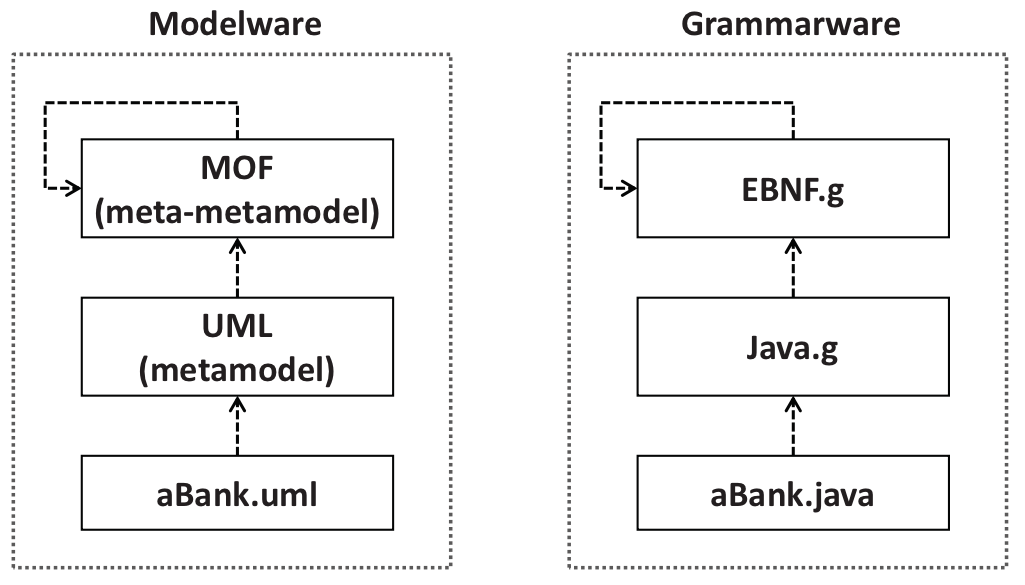
\includegraphics[scale=0.25]{figuras/modelWareVSGrammarWare}
\caption{Modelwarevs.Grammarware.}
\label{fig:modelWareVsGrammarWare}
\end{figure}

MDD é ainda considerado um paradigma atual no contexto de Engenharia de Software. MDD foi popularizado pela \textit{Object Management Group} (OMG) como \textit{Model Driven Architecture} (MDA)~\citep{Kleppe:2003}. Hoje em dia o Eclipse, o qual é um \textit{Integrated Development Environment}, é o ambiente padrão para MDD uma vez que o mesmo contêm uma implementação de referência do MOF, nomeado \textit{Eclipse Modeling Framework} (EMF).

\subsection{\textit{Model-Driven Reverse Engineering} (MDRE)}\label{sec:model_driven_reverse_engineering}

A utilização de MDD no contexto da ER (ou seja, MDRE) é um campo relativamente recente~\citep{Model_Driven_Reverse_Engineering}. No início, os modelos eram apenas utilizados, principalmente, para especificar os sistemas antes da sua implementação (durante a Engenharia Avante). MDRE propõe que modelos não sejam apenas artefatos que ``guiam'' o engenheiro durante tarefas de desenvolvimento e manutenção de software, mas como parte integrante do software~\citep{ThomasMDD}.


Devido ao grande interesse em MDRE, a OMG em 2003 inicio uma força tarefa (ADM \textit{taskforce}) que tinha como intuito padronizar o processo de engenharia reversa. Da mesma forma que MDA, a OMG criou a \textit{Architecture-Driven Mordernization} (ADM) que tem como objetivo criar especificações/padronizações para auxiliar processo de modernização de sistemas legados por meio de um conjunto de metamodelos padronizados. O fluxo de um processo de MDRE apoiada pela ADM possui três fases e é semelhante ao contorno de uma ferradura, são elas: Engenharia Reversa (ER) (do inglês, \textit{Reverse Engineering}), Reestruturação (do inglês, \textit{Restructuring}) e Engenharia Avante (EA) (do inglês, \textit{Forward Engineering}), como pode ser visto na Figura~\ref{fig:ADM_horse_shoes}. Partindo do lado inferior esquerdo, na parte da ER, o conhecimento é extraído do sistema legado e um modelo \textit{Plataform Specific Model} (PSM) é gerado. O modelo PSM serve como base para a geração de um modelo \textit{Platform Independent Model} (PIM), ou seja, durante a fase de ER, transformações são feitas como o intuito de se obter uma representação de alto nível do software, independentemente da plataforma utilizada anteriormente.

\begin{figure}[!ht]
\centering
  % Requires \usepackage{graphicx}
  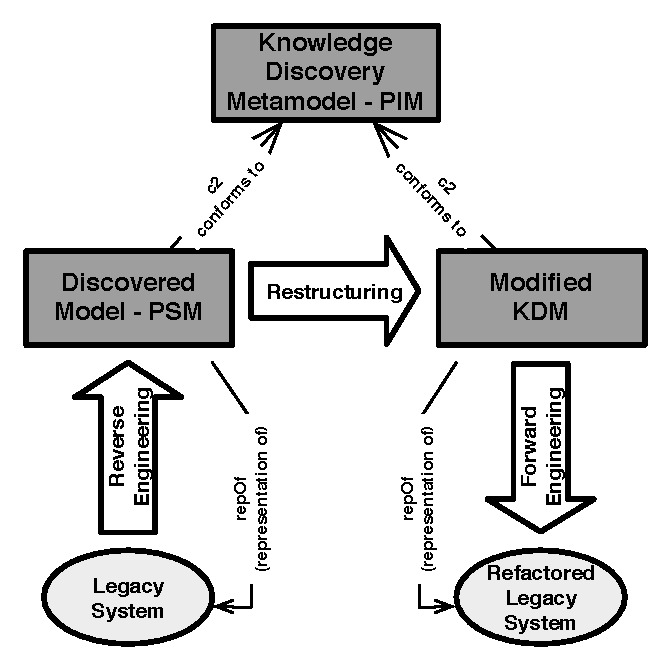
\includegraphics[scale=0.65]{figuras/horseShoe}
\caption{Fluxo do processo de modernização apoiada pela ADM (Adaptada~\citep{OMGADM})}
\label{fig:ADM_horse_shoes}
\end{figure}

O modelo PSM é um modelo especifico de uma plataforma, ou seja, nele existem metadados relacionados a uma plataforma ou linguagem de programação especifica. O modelo PIM é um modelo de abstração mais alto, pois não contém informações especificas de uma determinada plataforma ou linguagem.

Na fase de reestruturação, refatorações, melhorias e novas regras de negócios podem ser introduzidas no sistema, e, com uma representação independente de plataforma do software modernizado, segue-se para a fase de Engenharia Avante. Nessa ultima fase, os modelos são novamente submetidos a uma série de transformações para chegar ao nível de artefatos executáveis, ou seja, código-fonte.

No contexto da ADM, para dar suporte ao processo de modernização independentemente de plataforma e linguagem (PIM), foi criado um metamodelo que possibilita a comunicação entre diferentes plataformas e linguagens, e foi denominado pela ADM \textit{taskforce} de \textit{Knowledge Discovery Metamodel} (KDM)~\citep{ISOKDM}. O KDM provê representações para os sistemas de software existentes em diferentes camadas de abstrações. Cada modelo é representado por um conjunto de visões arquiteturais, ou seja, modelos KDM representando diferentes perspectivas de conhecimento sobre os artefatos dos sistemas de software existentes. Esses modelos são criados automaticamente, semi-automaticamente ou manualmente por meio da aplicação de várias técnicas de extrações de conhecimento, de análises e de transformações.~\citep{PerezCastillo:2011jo}.

O KDM representa artefatos físicos e lógicos de software dos sistemas legados em diferentes níveis de abstração e constitui dozes pacotes organizados em quatro camadas, são elas: infraestrutura (\textit{infrastructure}), elementos de programa (\textit{program elements}), recursos de tempo de execução (\textit{runtime resources}) e abstração (\textit{abstractions})~\citep{PerezCastillo:2011jo}. Na Figura~\ref{fig:KDMArchitecture} está representada a arquitetura do KDM ilustrando a forma como as camadas se relacionam. Cada camada baseia-se na camada anterior, dessa forma, elas estão organizadas em pacotes e definem um conjunto de metaclasses, cujo propósito é representar um interesse específico e independente do conhecimento relacionado a sistemas legados.

\begin{figure}[!ht]
\centering
  % Requires \usepackage{graphicx}
  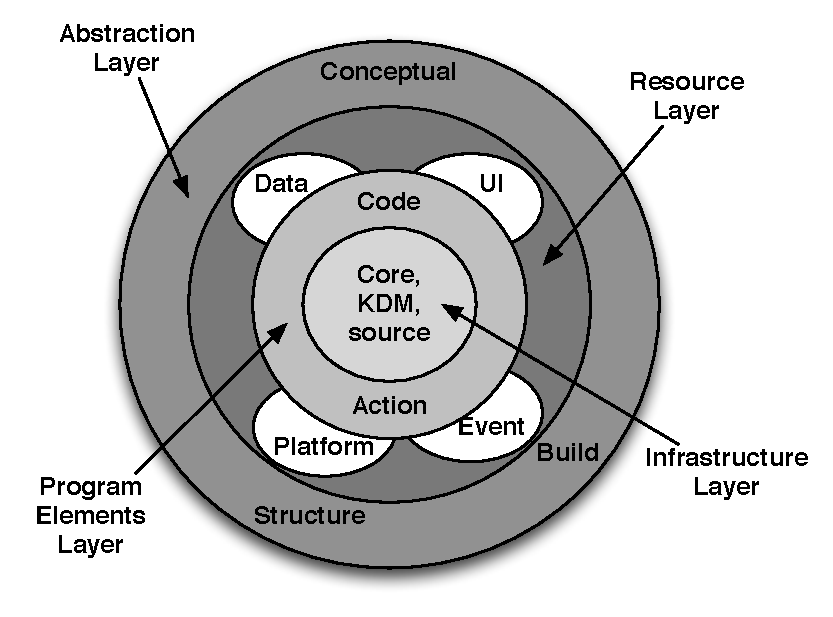
\includegraphics[scale=0.65]{figuras/Layers_packages_and_separations_of_concerns_in_KDM}
\caption{Arquitetura do KDM (adaptada~\citep{OMGADM})}
\label{fig:KDMArchitecture}
\end{figure}

Três pacotes importantes do KDM no contexto deste trabalho são: (\textit{i}) \textit{Code}, (\textit{ii}) \textit{Action} e (\textit{iii}) \textit{Structure}. Os dois primeiros pacotes contêm metaclasses para representar elementos de programação, tais como, classes, métodos, atributos, etc. Dessa forma, utilizando esses dois pacotes foi possível criar/adaptar um catalogo de refatoração para o contexto do KDM. Assim, todas as refatorações que foram adaptadas para o KDM agora são independentes de linguagem e plataforma. O terceiro pacote por sua vez (\textit{Structure}), define elementos de metamodelo que representam componentes arquitetural dos sistemas de software existentes. Por exemplo, esse pacote define as seguintes metaclasses: \textit{Subsystem}, \textit{Component}, \textit{Layer}, \textit{SoftwareSystem}, \textit{ArchitectureView}. Ressalta-se ainda que esse ultimo pacote, é de suma importância para as próximas atividades do outorgado, uma vez que verificação de conformidade em nível arquitetural serão implementadas para o KDM. Além disso, também serão definidas refatorações em nível arquitetural.

\subsection{Apoio ferramental}\label{sec:apoio_ferramental}

Diversas ferramentas de modelagem estão disponíveis para o desenvolvimento empresarial baseado em modelo, uma plataforma de ferramentas que se tornou proeminente no mundo da MDRE é o IDE Eclipse. Um conjunto de ferramentas interessantes para MDRE foram disponibilizados para essa IDE, permitindo, assim diversas iniciativas sobre esta plataforma. No contexto, do projeto em questão algumas iniciativas foram utilizadas: (\textit{i}) \textit{Eclipse Modeling Framework} (EMF), (\textit{ii}) Xtext, (\textit{iii}) Acceleo e (\textit{iv}) \textit{ATL Transformation Language} (ATL). 

\textit{Eclipse Modeling Framework} (EMF) é a principal iniciativa do IDE Eclipse no contexto de MDRE por várias razões. Primeiro, EMF permite a definição de metamodelos tendo como base uma linguagem de metamodelagem denominada Ecore. Em segundo lugar, EMF fornece um gerador de metamodelos, ou seja, uma API baseada em Java para manipulação de modelos. Em terceiro lugar, EMF contêm uma poderoso API que abrangem diferentes aspectos, tais como a serialização e deserialização de modelos de/para \textit{XML Metadata Interchange} (XMI). Xtext é um framework para desenvolvimento de Linguagens Específicas de Domínio (do inglês, \textit{Domain-Specific Language}). Acceleo é uma implementação pragmática do OMG para fornecer suporte a transformações \textit{Model2Text}. Por fim, ATL é uma linguagem de transformação de modelos, ou seja provê suporte a transformações \textit{Model2Model}. 










